\documentclass[twocolumn]{article}
\usepackage[a4paper, left=2cm, right=2cm, top=2cm, bottom=2cm]{geometry}
\usepackage{amsmath, amsthm, amssymb, esdiff, esint, indentfirst, longtable, array, dsfont, csquotes, fancyref}
\usepackage{graphicx}
\usepackage{titlesec}

\title{Special Function}
\author{Raffi C. Krisnanda}
\date{\today}

\titleformat{\section}[hang]{\bfseries}{\thesection.}{0.5em}{}
\titleformat{\subsection}[hang]{\bfseries}{\thesubsection.}{0.5em}{}
\DeclareMathOperator{\erfc}{erfc}
\DeclareMathOperator{\erfi}{erfi}
\DeclareMathOperator{\erf}{erf}

\begin{document}
\maketitle
\section{Gamma Function}
\subsection{Factorial.} The factorial is defined by integral
\begin{equation*}
    \int_{0}^{\infty} x^ne^{-\alpha x}\;dx=\frac{n!}{\alpha^{n+1}}
\end{equation*}
Putting $\alpha=1$ we get 
\begin{equation*}
    \int_{0}^{\infty} x^ne^{-x}\;dx=n!
\end{equation*}
Thus we have a definite integral whose value is $n!$ for positive integral $n$. We can also give a meaning to $0!$; by putting $n=0$, we get $0!=1$. By the way, the integral can be evaluated using differentiation under integral sign. 

\subsection{Gamma function definition.} Gamma function is used to define the factorial function for noninterger $n$. We define, for any $p > 0$
\begin{equation*}
    \Gamma(p)=\int_{0}^{\infty} x^{p-1}e^{-  x}\;dx
\end{equation*}

\subsection{Recursion relation.} The recursion for gamma function is 
\begin{equation*}
    \Gamma(p+1)=p\Gamma(p)
\end{equation*}
This can be used to define gamma function for $p\leq 0$
\begin{equation*}
    \Gamma(p)=\frac{\Gamma(p+1)}{p}
\end{equation*}

\emph{Proof.} Let us integrate $\Gamma(p+1)$ by parts. Calling $u=x^p$, and $ dv=e^{-x}\;dx$; then we get $du=px^{p-1}$, and $v=-e^{-x}$. Thus 
\begin{align*}
    \Gamma(p+1)&=-x^pe^{-x}\bigg|_0^{\infty}+\int_{0}^{\infty}e^{-x}px^{p-1}\;dx\\
    &=p\int_{0}^{\infty}x^{p-1}e^{-x}\;dx\\
    \Gamma(p-1)&=p\Gamma(p)\quad\blacksquare
\end{align*}

\subsection{Important formula.}
\begin{figure}[t]
    \centering
    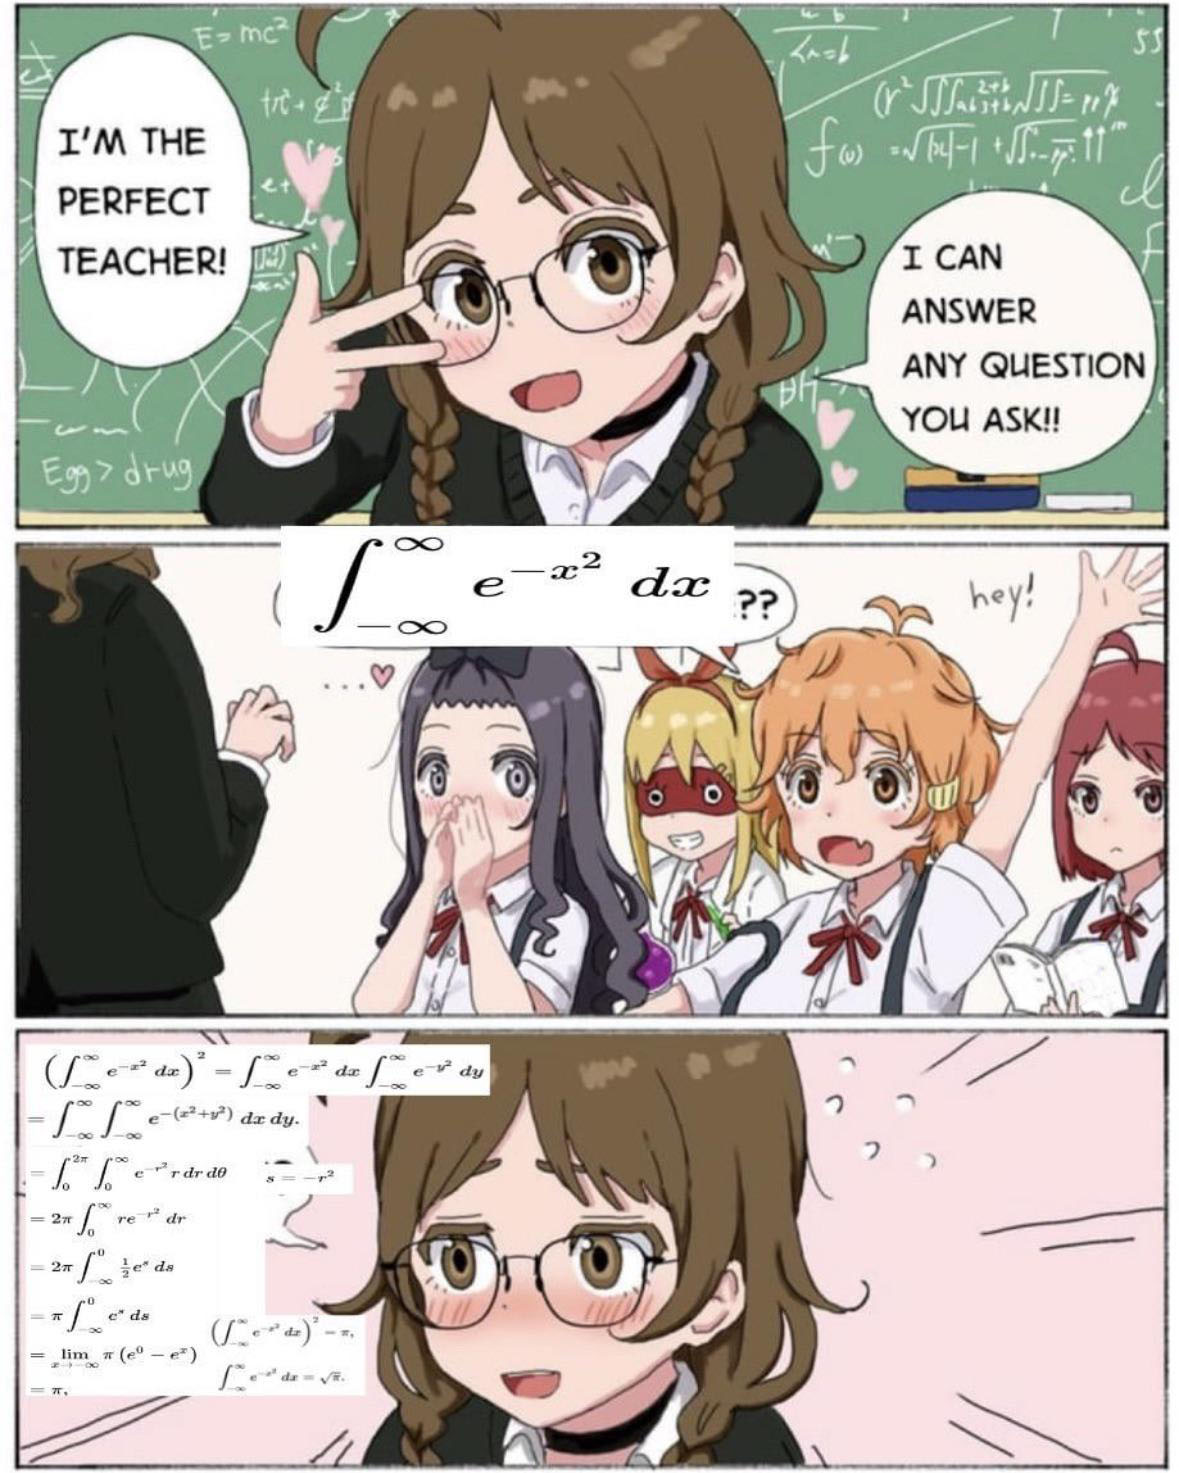
\includegraphics[width=\columnwidth]{./9az27w9ge34e1.jpg}
    \caption{Gaussian integral solved by polar method.}
    \label{fig}
\end{figure}
 We state here important formula
\begin{equation*}
    \Gamma(p)\Gamma(1-p)=\frac{\pi}{\sin \pi p}
\end{equation*}

We can calculate the value of $\Gamma(1/2)$ using this equation, however we will instead try to derive it using another method. First we consider the definition
\begin{equation*}
    \Gamma(1/2)=\int_{0}^{\infty}\frac{e^{-t}}{\sqrt{t}}\;dt
\end{equation*}
then we substitute $t=x^2$ and $dt=2x\;dx$
\begin{equation*}
    \Gamma(1/2)=2\int_{0}^{\infty}e^{-x^2}\;dx=\int_{-\infty}^{\infty}e^{-x^2}\;dx
\end{equation*}
This is the famous Gaussian integral. Refer to figure \ref{fig} on how to solve it solve it by polar coordinate. 


Since everybody and their grandma already know how to solve Gaussian integral by polar coordinate, I will instead try to solve it by Feynmann's trick. First consider the function
\begin{equation*}
    I(\alpha)=\biggl(\int_{0}^{\alpha}e^{-t^2}\;dt\biggr)^2
\end{equation*}
where $I$ is a function of parameter fish $\alpha$. Then, to evaluate the actual Gaussian integral
\begin{equation*}
    \int_{-\infty}^{\infty}e^{-x^2}\;dx=2\lim_{\alpha\rightarrow\infty}\sqrt{I(\alpha)}
\end{equation*}
Before that, I need to evaluate the function $I(\alpha)$ first. To do that, first I differentiate $I$ with respect parameter fish $\alpha$
\begin{align*}
    \frac{dI}{d\alpha}&=2\int_{0}^{\alpha}e^{-t^2}dt\biggl(\int_{0}^{\alpha}\frac{\partial e^{-t^2}}{d\alpha}\;dt+e^{-\alpha^2}\frac{d\alpha}{d\alpha}-e^{0}\frac{d(0)}{d\alpha}\biggr)\\
    \frac{dI}{d\alpha}&=\int_{0}^{\alpha}2e^{-(t^2+\alpha^2)}\;dt
\end{align*}
where I have used Leibniz' rule for differentiating under integral sign. Then, I introduce the variable $u=t/\alpha$ and $du=dt/\alpha$
\begin{equation*}
    \frac{dI}{d\alpha}=\int_{0}^{1}2e^{-(u^2\alpha^2+\alpha^2)}\alpha\;du=\int_{0}^{1}2\alpha e^{-\alpha^2(u^2+1)}\;du
\end{equation*}
Using the fact that
\begin{equation*}
    \frac{\partial}{\partial \alpha}\frac{e^{-\alpha^2(u^2+1)}}{u^2+1}=-2\alpha e^{-\alpha^2(u^2+1)}
\end{equation*}
I can rewrite the integrand as 
\begin{equation*}
    \frac{dI}{d\alpha}=-\int_{0}^{1}\frac{\partial}{\partial \alpha}\frac{e^{-\alpha^2(u^2+1)}}{u^2+1}\;du
\end{equation*}
Since the integrand is continous, I can move the partial differentiation outside the integral and turnig it into total differentiation
\begin{equation*}
    \frac{dI}{d\alpha}=-\frac{d}{d\alpha}\int_{0}^{1}\frac{e^{-\alpha^2(u^2+1)}}{u^2+1}\;du
\end{equation*}
Hence
\begin{equation*}
    I(\alpha)=-\int_{0}^{1}\frac{e^{-\alpha^2(u^2+1)}}{u^2+1}\;du+C
\end{equation*}
All that remains is to find the value of $C$. Considering the initial definition of $I(\alpha)$ and evaluating at $\alpha=0$, I get 
\begin{equation*}
    I(0)=\biggl(\int_{0}^{0}e^{-t^2}\;dt\biggr)^2=0
\end{equation*}
Therefore
\begin{align*}
    I(0)&=-\int_{0}^{1}\frac{1}{u^2+1}\;du+C=0\\
    C&=\arctan u\bigg|_{0}^{1}=\frac{\pi}{4}
\end{align*}
And I obtain the complete expression for the fish function
\begin{equation*}
    I(\alpha)=-\int_{0}^{1}\frac{e^{-\alpha^2(u^2+1)}}{u^2+1}\;du+\frac{\pi}{4}
\end{equation*}
Now I can evaluate the Gaussian integral
\begin{align*}
    \int_{-\infty}^{\infty}e^{-x^2}\;dx&=2\lim_{\alpha\rightarrow\infty}\biggl(-\int_{0}^{1}\frac{e^{-\alpha^2(u^2+1)}}{u^2+1}\;du+\frac{\pi}{4}\biggr)^{1/2}\\
    \int_{-\infty}^{\infty}e^{-x^2}\;dx&=2\frac{\sqrt{\pi}}{2}
\end{align*}
and I find 
\begin{equation*}
    \int_{-\infty}^{\infty}e^{-x^2}\;dx=\sqrt{\pi}
\end{equation*}

Much to my chagrin, it is actually more trouble some than the polar method. Let's us try it for comparison
\begin{equation*}
    \int_{-\infty}^{\infty}e^{-x^2}\;dx=\biggl(\int_{-\infty}^{\infty}\int_{-\infty}^{\infty}e^{-(x^2+y^2)}\;dx\;dy\biggr)^{1/2}
\end{equation*}
Doing the change of coordinate thing
\begin{align*}
    \int_{-\infty}^{\infty}e^{-x^2}\;dx&=\biggl(\int_{0}^{2\pi}\int_{0}^{\infty}e^{-r^2}r\;dr\;d\theta \biggr)^{1/2}\\
    \int_{-\infty}^{\infty}e^{-x^2}\;dx& = \biggl(2\pi\int_{0}^{\infty}e^{-r^2}r\;dr \biggr)^{1/2}
\end{align*}
That integral can by easily evaluated using $u$ substitution; making the substitution $u=-r^2$
\begin{align*}
    \int_{-\infty}^{\infty}e^{-x^2}\;dx &= \biggl(2\pi\int_{-\infty}^{0}\frac{e^u}{2}\;du \biggr)^{1/2}\\
    \int_{-\infty}^{\infty}e^{-x^2}\;dx & =  \biggl(2\pi\frac{e^u}{2}\bigg|_{-\infty}^{0} \biggr)^{1/2}
\end{align*}
And I get the same result 
\begin{equation*}
    \int_{-\infty}^{\infty}e^{-x^2}\;dx = \sqrt{\pi}
\end{equation*}
Damn, it is really more shrimple.

\section{Error Function} We define error function as 
\begin{equation*}
    \erf(x)=\frac{2}{\sqrt{\pi}}\int_{0}^{x}e^{-t^2}\;dt
\end{equation*}
There is also closely closely related integrals which are used and sometimes referred to as the error function called standard normal or Gaussian cumulative distribution function $\Phi(x)$
\begin{equation*}
    \Phi(x)=\frac{1}{\sqrt{2\pi}}\int_{-\infty}^{x} e^{-t^2/2}\;dt
\end{equation*}
Here are some of their relations.
\begin{align*}
    \Phi(x)&=\frac{1}{2}+\frac{1}{2}\erf\bigl(x/\sqrt{2}\bigr)\\
    \Phi(x)-\frac{1}{2}&=\frac{1}{2}\erf\bigl(x/\sqrt{2}\bigr)\\
    \erf(x)&=2\Phi\bigl(x\sqrt{2}\bigr)-1
\end{align*}

\emph{Proof.} Consider the definition of $\Phi(x)$. Making the substitution of $u=t/\sqrt{2}$
\begin{align*}
    \Phi(x)&=\frac{1}{\sqrt{2\pi}}\int_{u=-\infty}^{u=x/\sqrt{2}}e^{-u^2}\sqrt{2}\;du\\
    &=\frac{1}{\sqrt{\pi}} \biggl(\int_{-\infty}^{0}e^{-u^2}\;du+ \int_{0}^{\infty}e^{-u^2}\;du\biggr)\\
    \Phi(x)&=\frac{1}{2}+\frac{1}{2}\erf\bigl(x/\sqrt{2}\bigr)\quad\blacksquare
\end{align*}
To prove the third relation, we first rewrite the equation as
\begin{align*}
    \erf\bigl(x/\sqrt{2}\bigr)= 2\Phi(x)-1
\end{align*}
then we make the substitution $u=x/\sqrt{2}$
\begin{align*}
    \erf(u)&= 2\frac{1}{\sqrt{2\pi}}\int_{-\infty}^{u\sqrt{2}} e^{-t^2/2}\;dt-1\\
    \erf(u)&=2\Phi\bigl(x\sqrt{2}\bigr)-1\quad\blacksquare
\end{align*}

\subsection{Complementary error function.} Defined as 
\begin{equation*}
    \erfc(x)=\frac{2}{\sqrt{\pi}}\int_{x}^{\infty}e^{-t^2}\;dt
\end{equation*}
It relations with the actual error function are as follows.
\begin{align*}
    \erfc(x)&=1-\erfc(x)\\
    \erfc\big(x/\sqrt{2}\big)&=\sqrt{\frac{2}{\pi}}\int_{x}^{\infty}e^{-t^2/2}\;dt
\end{align*}

\emph{Proof.} The first relation is quite easy to prove. Consider
\begin{equation*}
    \frac{2}{\sqrt{\pi}}\int_{-\infty}^{\infty}e^{-t^2}\;dt=1
\end{equation*}
then
\begin{align*}
    \frac{2}{\sqrt{\pi}}\biggl(\int_{-\infty}^{x}e^{-t^2}+\int_{x}^{\infty}e^{-t^2}\biggr)&=1\\
    \erf(x)+\erfc(x)=1\quad\blacksquare
\end{align*}
To proof the second relation, we subtitute the limit of integration from $t=x/\sqrt{2}$ into $x=t\sqrt{2}$
\begin{align*}
    \erfc\bigl(x/\sqrt{2}\bigr)&=\frac{2}{\sqrt{\pi}}\int_{x}^{\infty}\frac{e^{t^2/2}}{\sqrt{2}}\;dt\\
    \erfc\bigl(x/\sqrt{2}\bigr)&=\sqrt{\frac{2}{\pi}}\int_{x}^{\infty}e^{-t^2/2}\;dt\quad\blacksquare
\end{align*}

\subsection{Imaginary error function.} We define
\begin{equation*}
    \erfi(x)=\frac{2}{\sqrt{\pi}}\int_{0}^{x}e^{t^2}\;dt
\end{equation*}
Here are some relation to the actual error function.
\begin{align*}
    \erf(ix)&=i\erfi(x)\\
    \erf\biggl(\frac{1-i }{\sqrt{2}}x\biggr)&=(1-i   )\sqrt{\frac{2}{\pi}}\int_{0}^{x}(\cos^2u+i\sin^2u)\;du
\end{align*}
\end{document}
